\chapter{Statistics: what it is and why it works}

\section{Motivation}

By now, we have learned a whole lot about probability theory. In the previous chapter we have seen
how to compute the distribution of a RV given another RV. Moreover, we know how to factor joint distributions and simplify them by making
independence assumptions. In principle, this puts us in a good position to start formulating our
own probabilistic models. However, our models will be pretty useless if we do not know their parameters. And as
it so happens, we virtually never know them in real life. So what we are going to talk about next is how to \textbf{estimate}
these parameters from data that we observe. The tools we are going to use for estimation come from statistics.

Statistics is a relatively broad term. There are many ways of doing it and chances are that different people from different
fields mean different things when they use the term \textit{statistics}. This is mostly so because the goals that people 
want to achieve using statistics are different. The underlying mechanics do in fact not differ that much. In this course,
we are going to focus on the basics of statistics that you need to know no matter what your goals are. However, allow us
to give you a quick birds-eye view on statistics. 

There are two main goals you can have using statistics (this is grossly oversimplified, but hey, we said it was the birds-eye
view). On the one hand you can do \textbf{descriptive statistics} which means that you are gathering information about a phenomenon
that you are interested in and report that information. For example, you might be interested in how many faculty members
at your university are alcoholics. What you do is you go to each faculty member, check whether they are an alcoholic
and report the total number of alcoholics at your institute. Crucially, you are not going to draw any conclusions (such as that people working in the humanities are more
likely to be alcoholics than those working at the science faculty).

Another, somewhat milder example of descriptive statistics are housing advertisements. If you are looking for a flat, you will usually
find descriptions of the offered flats in terms of square metres, storey, the presence of a balcony, etc. All of these descriptions
can be seen as descriptive statistics. Again, when reviewing these ads, your goal will not be to make a statement like "flats
with a balcony are more habitable than flats without one". This may be your own preconception, but it is nothing that
you would be trying to get out of your data.

The second big part of statistics is \textbf{inferential statistics}. Here you are actually interested in drawing
conclusions (inferences). So if you do an alcoholism survey amongst faculty at your university, you would like to find some
way of determining the relationship between area of research, say, and the chance that someone is an alcoholic. The rest of the
course will mostly be about inferential statistics. In particular, our main question will be the following: given that we observe some data and
we know (or assume) that the data is distributed according to some distribution (e.g.\ a multinomial) what are the parameters of that distribution? Hence, we will try to infer the parameters.

Within inferential statistics, there is a further distinction one can make. In \textbf{statistical (data) analysis} people are interested in analysing
the properties of a given data set. Say you have obtained questionnaires from 500 faculty members. Then your goal is to make
statements about these 500 questionnaires. The scope of your study does not extend beyond those 500 data points and all statements that you make
are in principle limited to this data set. Obviously, this is not what people do in research papers. Researchers
often try to generalize the results they obtain on their data set to a bigger population, like all university employees or even
all of humankind. In the following sections we are going to give some indication for why such generalisations may be justified and
at the same time warn you that they are often not.

Finally, there is the field of \textbf{prediction}. In prediction you again analyse your data, but what you actually want to
do is to predict future data of the same kind. Your current data set is of no actual interest to you except that it allows you
to gather information that may turn out to be valuable for making your predictions. Again, if you have compiled 500 questionnaires from 
faculty, you would like to predict what the rate of alcoholics for the following 100 questionnaires is. After you have extracted
the information you need from your original data set, you could even discard it in this setting. In practice, of course, you 
should NEVER discard your data. Instead, you should make it publicly available, so that other people can reproduce your study.

This latter field of prediction is nowadays most commonly known as \textbf{machine learning}. However, statistical analysis and 
prediction are closely intertwined and share a lot of their methodology. It is therefore not always easy to make the distinction.


\section{Statistics and Sample Means}

In the previous section we have introduced the word \textbf{statistic} and also alluded to the fact that we often assume that our
observed data is distributed according to some distribution. The way we usually conceptualize data is that each data point is
an instantiation of a random variable. This means that when you are observing 1000 data points, we conceptualize this as observing
the outcomes of 1000 random variables. Importantly, each data point could potentially have taken on a different value and it just 
so happens that in our specific \textbf{data sample} it took on the value that it did. 

There is one further assumption that we usually make about our data, namely that it is \textbf{i.i.d.}\ (identical and independently
distributed). This just means that we assume that all the random variables that generated our data points follow the same distribution and 
that they are independent of each other. When we say they follow the same distribution, we do not just mean the same class of
distributions (e.g.\ multinomial), but really the same distribution with identical parameters. We often
call that distribution the \textbf{data-generating distribution}, but you also find the terms 
\textit{underlying distribution} or \textit{true distribution} in the literature. 
We have in fact already used the i.i.d.\ assumption before. When we do repeated Bernoulli trials (as in Section~\ref{sec:importantdistributions}), the total probability of the resulting sequence is computed as a product
of independent RVs. We can encode the i.i.d.\ assumption for $ n $ Bernoulli trials as follows:
\begin{equation}
\forall i \ \mbox{s.t.} \  1 \leq i \leq n : X_{i} \sim Bernoulli(\theta) \, .
\end{equation}

All $ X_{i} $ follow the same distribution since the parameter $ \theta $ does not depend on $ i $ but is constant throughout.
By the same token, we get independence as the distribution does also not depend on other RVs. Thus, repeated Bernoulli trials,
such as repeated coin flips, do actually invoke the i.i.d.\ assumption. When working with real data this assumption will often be
violated but we are going to make it nonetheless for mathematical convenience or if we can motivate it
based on our knowledge of the data set.

After we have described our conception of data, let us move on to defining what a statistic is.

\begin{Definition}
A \emph{statistic} is the value of any function of a data sample. If we have sampled $ n $ data points that we assume are instantiations of RVs
$ X_{1}^{n} $, a statistic is the value of a function $ g $ on those RVs, i.e.\ $ g(X_{1}^{n}) $.
\end{Definition}

Arguably the most important statistic in all of statistics is the \textbf{sample mean}. The sample mean is just the average of the
values of the RVs $ X_{1}^{n} $, i.e.\ of the data points. It is usually denoted by $ \overline{\mu} $. The
sample mean can be seen as guess of the expectation of $ X_{i} $. The expectation is sometimes also
called mean and $ \overline{\mu} $ estimates it from a data sample; hence the name sample mean. Some distributions even have their
mean $ \mu $ as a parameter. To indicate that we are just making a guess at $ \mu $ we put a horizontal bar on top.
This same indicator (or a similar one, like a caret, in which case we would write $ \hat{\mu} $) can be used for other quantities, as well.

\begin{Definition}
The sample mean of i.i.d.\ random variables $ X_{1}, \ldots, X_{n} $ is defined as 
$$ \overline{\mu} := \dfrac{1}{n}\underset{i=1}{\overset{n}{\sum}} X_{i} \ . $$
\end{Definition}

Notice that since $ \overline{\mu} $ is the average of a collection of random variables, it is itself a random variable. Thus, we can
compute its expectation.
\begin{align}
\E[\overline{\mu}] &= \E\left[\dfrac{1}{n} \underset{i=1}{\overset{n}{\sum}} X_{i}\right] \label{eq:sampleMeanBegin} \\
&= \dfrac{1}{n} \E\left[\underset{i=1}{\overset{n}{\sum}} X_{i}\right] \label{sampleMeanStep1} \\
&= \dfrac{1}{n} \times n \E[X] \label{sampleMeanStep2} \\
&= \E[X] = \mu \label{eq:sampleMeanEnd}
\end{align}

This result is huge! Before we interpret it, let us be clear about how we computed it: lines \eqref{sampleMeanStep1} and
\eqref{sampleMeanStep2} follow from the linearity of expectation and the fact that the RVs are i.i.d. 

So why is this result so important? It says that the expectation of the sample mean is equal to the true
mean. This means that sampling data gives us a way to estimate the true mean. Since the sample means are random variables and therefore distributed according
to some distribution, each sample mean should show up in proportion to its probability. Thus, the mean
of sample means will approximate the true mean. Conceptually this may be quite a bit to chew on, but the practical implications are compelling.
If you are running one experiment (i.e.\ if you take one data sample) you basically have no clue how probable that sample mean is according
to the distribution of sample means. It could be very improbable and thus not be representative at all of the population you are investigating.
So what should you do? The above result tells us that you should just repeat your experiment \textit{enough} times, so that you get
\textit{enough} sample means. The mean of those sample means will in turn be pretty close to the true mean of the distribution that underlies your population
of interest. This is the mathematical reason why in science we want our experimental results to be replicable. If I get a result
and several other people get the same or reasonably close results, we can be fairly sure that we obtained them from a high-probability region
in the distribution of sample means, i.e.\ the results are indeed representative for the population under scrutiny.

\begin{Exercise}
Under \href{https://github.com/BasicProbability/LectureNotes/blob/master/chapter5/BernoulliData.txt}{this link} you find a file that contains 1000 random samples from
a binomial distribution with parameter $ n = 100 $. The file contains 1000 numbers and the i$ ^{th} $ number is number of successes in the i$ ^{th} $ sample. Write
a Python script that computes an approximation to the parameter $ \theta $ of the binomial.
\end{Exercise}

We have just said that repetition of results is the gold standard in science because if several sample means
are close to each other, each one of them (and their average) is likely to be a reasonable approximation
to the true mean of the underlying distribution. Unfortunately, more often than not, we only draw
one data sample and thus only have one sample mean. The natural question to ask is whether we can
somehow ensure that this one sample mean is informative about the true mean. The strict answer is no.
We can always be unlucky and obtain a very improbable and thus non-representative sample mean. On the bright
side, we can take measures to reduce or chance of being unlucky (and thereby make the one sample mean more
trustworthy). What these measures are is explained in Section~\ref{LawOfLargeNumbers}. Let us first
review the concept of limits in preparation for the proofs that we are going to see in that Section.

\section{Limits}
To help our understanding of the theorem in Section~\ref{LawOfLargeNumbers} we have to recall how mathematical limits are defined. For an infinite sequence of numbers we can ask ourselves whether the sequence will eventually come close to a single point or whether it will just keep moving through the space of real numbers. This
question can be formalized with the concept of limits.

\begin{Definition}[Finite Limit of a sequence]\label{def:finiteLimit}
Take any sequence of real numbers $ \left( a_{n} \right) $ where $ a_{n} : = a(n) $ for some function $ a : \mathbb{N} \rightarrow \mathbb{R} $.
We say that $ L \in \mathbb{R} $ is the \emph{limit} of that sequence as $ n $ goes to infinity if for any $ \eps > 0 $ we can find an 
$ n_{0} \in \mathbb{N} $ such that for any $ n \geq n_{0} $
$$ |L - a_{n}| \leq \eps\ . $$
We write $ \underset{n \rightarrow \infty}{\lim} a_{n} = L $ to express this fact.
\end{Definition}

\begin{Definition}[Infinite Limit of a sequence]\label{def:infiniteLimit}
Take any sequence of real numbers $ \left( a_{n} \right) $. We say that the sequence diverges (to $ \pm \infty $) if for every $ K \in \mathbb{R} $ there is 
an $ n_{0} \in \mathbb{N} $ such that for all $ n > n_{0} $ it holds that
$$ |a_{n}| \geq K \ . $$
We write $ \underset{n \rightarrow \infty}{\lim} a_{n} = \pm \infty $ to express this fact.
\end{Definition}

Definition~\ref{def:finiteLimit} tells us that if a sequence converges to a limit $ L $, then for all but finitely many elements (those at the beginning of the sequence)
the difference between each element and $ L $ will be $ \leq \eps $. More informally, we can say that the difference between the elements of the sequence and $ L $
can be made arbitrarily small if we are willing to walk far enough down the sequence. Definition~\ref{def:infiniteLimit} has been included for completeness' sake but will 
not be of much relevance in the remainder of the course. 

Notice that it is possible that a sequence has no limit at all (neither finite nor infinite). We will not deal with this case here, though. 

\paragraph{Example of a limit calculation}
To give you some more feeling for limits, here is an example. Consider the sequence $ a_{n} = \frac{1}{n} $. What is its limit? Intuitively, $ a_{n} $ becomes smaller
as $ n $ becomes larger. Moreover, all $ a_{n} $ are non-negative. A good guess for the limit thus seems to be $ L = 0 $. Let us show that it is indeed the limit of this
sequence. Choose any real $ \eps > 0 $. Then for $ n \geq n_{0} $ we want that 
\begin{equation} \label{limitexample}
|L - a_{n}| = |a_{n}| = \dfrac{1}{n} \leq \eps\
\end{equation}
We solve this inequality to get $ n \geq \nicefrac{1}{\eps} $. Thus we set $ n_{0} = \lceil \nicefrac{1}{\eps} \rceil $ which is the smallest integer $n_0 \in \mathbb{N}$ such that $\nicefrac{1}{\eps} \leq  n_0$. Since $ \eps $ was chosen arbitrarily we conclude
that indeed $ \underset{n \rightarrow \infty}{\lim} \frac{1}{n} = 0 $. $ \square $\bigskip

Instead of limits of sequences, we will actually need limits of functions. However, notice that limits of functions are simply the limits of sequences of function
outputs. 

\begin{Definition}[Limit of a function]
Consider a function $ f $ that is defined on the reals. We say that the limit of $ f(x) $ as $ x $ approaches $ x_{0} $ is $ L $ if for every $\eps >0$ there exists a $\delta >0$ such that $0<|x-x_0| \leq \delta$ implies
$$  |L - f(x)| \leq \eps \ .$$
We write $ \underset{x \rightarrow x_{0}}{\lim} f(x) = L $ to express this fact.
\end{Definition}

\section{The Weak Law of Large Numbers}\label{LawOfLargeNumbers}
The weak law of large number states that as we increase our sample size, the probability tends to 0 that our estimated mean $ \overline{\mu} $ will be further than a small
amount $ \eps $ away from the true expectation $ \E[X] $ of the data-generating distribution $ P_{X} $. In other words, the more sample points we take, 
the smaller is the chance that we commit a large error when estimating the mean from our sample. To become clear about what we need to prove, let us first state
the weak law of large numbers.

\begin{Theorem}[Weak law of large numbers]\label{weakLaw}
For $n \in \mathbb{N}$, let $X_{1}^{n},$ be  i.i.d.\ distributed random variables with distribution $ P_{X} $, expectation $ \E[X] \in \mathbb{R} $
and variance $ var(X) = \sigma^{2} \in \mathbb{R} $. Further let
$ X_{1}^{n} $ have sample mean $ \overline{\mu} = \frac{1}{n} \underset{i=1}{\overset{n}{\sum}X_{i}} $. Then for any real $ \eps > 0 $, it holds that 
$$ \underset{n \rightarrow \infty}{\lim}P(|\mathbb{E}[X] - \overline{\mu}| \geq \eps) = 0 \ . $$
\end{Theorem}

At this point it may be good to just pause for a moment, stare at the theorem and try to connect it to the verbal explanation from above. The significance of the theorem
derives from the fact that it basically provides us with the theoretical underpinning that allows us to draw inferences from data.

In order to prove the weak law of large numbers, we use two auxiliary lemmas. Once we have proven those, Theorem~\ref{weakLaw} will follow easily. 

\begin{Lemma}[Markov's inequality]\label{markovIneq}
For any random variable $ X $ and any $ a \in \mathbb{R} $ it holds that
$$ P(|X| \geq a) \leq \dfrac{\mathbb{E}[|X|]}{a} \ . $$
\end{Lemma}

\begin{Exercise}
Prove Markov's inequality.
\end{Exercise}

Besides having established Lemma~\ref{markovIneq}, \href{https://en.wikipedia.org/wiki/Andrey_Markov}{Andrey Markov} has made many significant contributions to
probability theory. For example, if you go on to study information theory and/or any computational linguistics courses, you are guaranteed to encounter \href{https://en.wikipedia.org/wiki/Markov_chain}{Markov chains}. For now, let us move on to our second auxiliary lemma.

\begin{Lemma}[Chebyshev's inequality]\label{Chebyshev}
Let $ X $ be a RV with expectation $ \mathbb{E}[X] $ and variance $ var(X) = \sigma^{2} \in \mathbb{R} $. Furthermore, let $ \eps > 0 $. Then
$$ P( \left|\mathbb{E}[X] - X \right| \geq \eps) \leq \dfrac{\sigma^{2}}{\eps^{2}} \ . $$ 
\end{Lemma}

\paragraph{Proof of Lemma~\ref{Chebyshev}} 
By Markov's inequality we have that
\begin{equation}
P((\mathbb{E}[X] - X)^{2} \geq \eps^{2}) \leq \frac{\E[(\E[X]-X)^2]}{\eps^2} = \dfrac{var[X]}{\eps^{2}} = \dfrac{\sigma^{2}}{\eps^{2}} \ .
\end{equation}  
\hfill $ \square $ \bigskip

The final step in proving the weak law of large numbers is to apply Chebyshev's Inequality in the case where the random variable of interest is
the sample mean.

\paragraph{Proof of Theorem~\ref{weakLaw}} We assume i.i.d.\ RVs $ X_{1}^{n} $ with sample mean $ \overline{\mu} = \frac{1}{n} \underset{i=1}{\overset{n}{\sum}} X_{i} $. 
This means that $ \mathbb{E}[X] - \overline{\mu} $  is a RV depending on $ X_{1}^{n} $ whose variance is
\begin{align}
var(\mathbb{E}[X] - \overline{\mu}) &= var(\overline{\mu}) \\ 
&= var\left(\frac{1}{n} \underset{i=1}{\overset{n}{\sum}} X_{i} \right) \\
&= \frac{1}{n^{2}}var\left(\underset{i=1}{\overset{n}{\sum}} X_i\right) \\
&= \frac{1}{n^{2}}~n~var(X) = \dfrac{var(X)}{n} \ .
\end{align}
Chebyshev's Lemma~\ref{Chebyshev} then implies that 
\begin{equation}
\underset{n \rightarrow 0}{\lim}P(|\mathbb{E}[X] - \overline{\mu}| \geq \eps) \leq \frac{\sigma^{2}}{n\eps^{2}} \ .
\end{equation}

If we fix $ \eps > 0 $ and increase $n$, the number of i.i.d.\ samples, this probability will go to 0.
More formally, choose $ \delta > 0 $. One way to show $ P(|\mathbb{E}[X] - \overline{\mu}| \geq \eps) $ to be smaller than $ \delta $, is to show 
$ \frac{\sigma^{2}}{n\eps^{2}} < \delta $ which happens whenever $ \frac{\sigma^{2}}{\delta\eps^{2}} < n $. Thus, if we sample
more than $ \frac{\sigma^{2}}{\delta\eps^{2}} $ data points, we can ensure that $ P(|\mathbb{E}[X] - \overline{\mu}| \geq \eps) < \delta $.
Since $ \delta $ is arbitrary, this shows that $ \underset{n \rightarrow \infty}{\lim}~P(|\mathbb{E}[X] - \overline{\mu}| \geq \eps) = 0 $, 
which is exactly what the weak law of large numbers states. $ \square $ \bigskip

The proof of the weak law of large numbers also sheds some new light on the importance of the variance of the underlying distribution. 
We want that variance to be as small as possible
since we then need fewer samples in order to have a close estimate of the true mean of the data-generating distribution. 
Thus, it is helpful if the variance of the 
data-generating distribution is small. Otherwise we need a lot of samples.

Notice also the relationship between the variance $ \sigma^{2} $ and the number of samples $ n $ in the above proof. For a fixed variance, the
probability $ P(|\mathbb{E}[X] - \overline{\mu}| \geq \eps) $ reduces by a factor that is proportional to $ n $. Hence, we need to take
more and more samples as we want to decrease the probability that the sample mean deviates from the actual mean by more than $ \eps $. 

A more common and more practical interpretation of the relationship between $ \sigma^{2} $ and $ n $ is the following: suppose we have collected $ n $ data
points where $ n $ is fixed, meaning we have no quick and cheap way to obtain more data points. Then the lower the variance of the data-generating distribution, 
the more confident we can be
that $ \overline{\mu} $ is a reasonably good estimate of the true mean of the data-generating distribution. This insight also establishes a relationship to
the expectation of sample means (see Equations~\eqref{eq:sampleMeanBegin}-\eqref{eq:sampleMeanEnd}). If the distribution of sample means has low variance, the
interval of sample means that are likely to occur is relatively tight. Thus we will only need few sample means in order to compute a good approximation to
the true mean.

To visualise the effect of the sample size for a fixed variance, 
let us take a look at Figure~\ref{fig:likelihood_plots}. The plot on the top shows the same function applied
to different data samples from the same distribution, all of which are of relatively small size. 
The plots therefore show large spread as witnessed by the width of the curves. The 
plot at the bottom shows the same function applied to a larger data set. One clearly sees that the spread is much smaller.

\section{Sufficient Statistics}\label{sec:sufficientStats}

A popular interpretation of statistics is that they are data summaries. Obviously, some statistics summarize
the data better than others. For example, the constant function $ \mathbf{6}(\cdot) $ which returns the
value 6 on all inputs delivers an extremely poor summary of most data (in fact it is not sensitive to the
data at all). The mean is a more useful summary as it captures some overall tendency in the data. 

Is there any statistic that captures all the necessary information in the data? This questions is hard
to answer in general but when it comes to capturing the information about the parameters of the
underlying distribution, the answer is yes\footnote{At least for the distributions that we are 
concerned with in this script, which are all in the \href{https://en.wikipedia.org/wiki/Exponential_family}{exponential family}.}. If a statistics
conveys all the information about the parameters that the data contain, we call it a \textbf{sufficient
statistic}. The formal definition is somewhat less obvious.

\begin{Definition}[Sufficient Statistics (discrete)]\label{def:discreteSuffStat}
Given some discrete RV $ X $ over data and a statistical model with parameters $ \theta $, 
a statistic $ t(x) $ is sufficient if $ P(X=x|t(X) = t(x), \Theta = \theta) $ does not depend on $ \theta $,
i.e. if 
$$ P(X=x|t(X) = t(x), \Theta = \theta) = P(X=x|t(X) = t(x)) \ . $$
\end{Definition}

The above definition captures exactly what it means for a statistic to contain all the information
about the parameters. Once we know the sufficient statistic, we can simply ignore the parameters. As an
example, consider the Bernoulli distribution. For set of i.i.d Bernoulli trials $ x=x_{1}^{n} $,
the statistic $ t(x) = \sum_{i=1}^{n} x_{i} $ is sufficient. To see this, consider the distribution
$ P(X|\sum_{i=1}^{n} x_{i}, \Theta = \theta) $. It takes the following form
\begin{equation*}
P\left( X=y|\sum_{i=1}^{n} x_{i}, \Theta = \theta \right) = 
\begin{cases}
0 & \mbox{if } \sum_{i=1}^{n} y_{i} \not = \sum_{i=1}^{n} x_{i} \\
\frac{1}{\binom{k}{n}} & \mbox{otherwise, where } k = \sum_{i=1}^{n} x_{i}
\end{cases}
\end{equation*}
Clearly, neither of the two left-hand-side terms depends on $ \theta $. Thus, $ t(x) = \sum_{i=1}^{n} x_{i} $
is a sufficient statistic according to our definition. Notice that the sum does not capture the
order in which the events occurred. This shows that the sufficient statistic is not a perfect summary
in general (after all, we might care about the order of events). It only captures all the information
about the parameters that the data contain.

A statistic that is non-sufficient for the Bernoulli distribution is the value of the first outcome, i.e.\ 
$ t(x) = x_{1} $. There are several binary sequences that have the same starting value but
different numbers of ones and zeros. The corresponding conditional distribution is
\begin{equation*}
P(X=y|x_{1}, \Theta = \theta)
\begin{cases}
= 0 & \mbox{ if } y_{1} \not = x_{1} \\
\propto \binom{k}{n} \theta^{k} (1 - \theta)^{n-k} & \mbox{ otherwise, where } k = \sum_{i=1}^{n} x_{i}
\end{cases}
\end{equation*}
where the proportionality follows because we need to renormalise the probability to all those
sequences whose starting values is equal to $ x_{1} $. The crucial point, however, is that the parameter
shows up in the right hand side and thus $ x_{1} $ is not a sufficient statistic for the binomial
distribution.

\begin{Exercise}
Assume a RV $ X=X_{1}^{n} $ whose observations are i.i.d. according to a Poisson distribution
with parameter $ \lambda $. Recall that the p.m.f. of the Poisson distribution for one data point is
$$ P(X=x|\Lambda = \lambda) = e^{-\lambda}\frac{\lambda^{x}}{x!} \ . $$
Show that $t(x) = \sum_{i=1}^n x_i$ is a sufficient statistic for the Poisson distribution as well.
\end{Exercise}

Definition~\ref{def:discreteSuffStat} is constrained to discrete distributions. It is also not very useful
when one does not yet know the sufficient statistics and has to find them. We will remedy both these problems
with the following theorem.
\begin{Theorem}[Factorisation Theorem]
Assume a discrete RV over data $ X $ and a statistical model $ P(X=x|\Theta=\theta) $ with parameters $ \theta $.
A statistic $ t(X) $ is sufficient if and only if the model can be written as
$$ P(X = x | \Theta = \theta) = g(\theta, t(x)) \cdot h(x, t(x)) \ . $$
\end{Theorem}
\paragraph{Proof} Assume $ t(x) $ is sufficient. Then
\begin{align}
P(X = x | \Theta = \theta) &= P(X=x, t(X)=t(x) | \Theta = \theta) \label{eq:fact1}\\ 
&= P(X=x|t(X) = t(x), \Theta=\theta) \cdot P(t(X) = t(x)| \Theta = \theta)\\
&= P(X=x|t(X) = t(x)) \cdot P(t(X) = t(x)| \Theta = \theta) \label{eq:fact2}\\
&= h(x, t(x)) \cdot g(\theta, t(x)) \ , \nonumber
\end{align}
where in~\eqref{eq:fact1}, we used the fact that $t(\cdot)$ is a deterministic function, the second equality is the chain rule and in~\eqref{eq:fact2}, we use that $t(x)$ is sufficient.
Now assume that $ P(X = x | \Theta = \theta) = g(\theta, v(x)) \cdot h(x, v(x)) $ for some statistic $ v(x) $. We need to show
that $ v(x) $ is sufficient in the sense of Definition~\ref{def:discreteSuffStat}. Observe that $ P(X=x,V(X)=v(x)|\Theta = \theta) = P(X=x|\Theta = \theta) $
since $ v(\cdot) $ is deterministic. Thus
\begin{align}
&P(v(X)= v| \Theta = \theta) = \sum_{x:v(x)=v}P(X=x,v(X)=v| \Theta = \theta) \\
&= \sum_{x:v(x)=v}P(X=x | \Theta = \theta) = \sum_{x:v(x)=v} g(v, \theta) h(x,v) \nonumber
\end{align}
where the last equality follows from our assumption that the p.m.f. of $ X $ can be rewritten in the desired way. We now use the p.m.f. for $ v(x) $
in the next step.
\begin{align}
&P(X=x|v(X) = v, \Theta=\theta) = \dfrac{P(X=x,v(X)= v|\Theta = \theta)}{P(v(X) = v|\Theta = \theta)} \\
&= \dfrac{P(X=x|\Theta = \theta)}{P(v(X) = v|\Theta = \theta)}  \\
&= \frac{g(\theta, v)h(x, v)}{\sum_{x:v(x)=v} g(v, \theta) h(x,v)}
= \frac{h(x, v)}{\sum_{x:v(x)=v} h(x,v)}
\end{align}
Clearly, the conditional does not depend on $\theta $ and thus $ v(X) $ is sufficient. $ \square $ \bigskip


Now that we have shown the factorisation theorem for discrete RVs we will use it as a general definition for sufficiency, thereby
also including continuous RVs.
\begin{Definition}[Sufficient Statistic]
Given some RV $ X $ over data and a statistical model with parameters $ \theta $, 
a statistic $ t(x) $ is sufficient if $ P(X=x|t(X) = t(x), \Theta = \theta) $ can be written as
$$ P(X = x | \Theta = \theta) = g(\theta, t(x)) \cdot h(x, t(x)) \ . $$
\end{Definition}

\section{Parameter Estimation}\label{parameterEstimation}

It is time for us to meet \href{https://en.wikipedia.org/wiki/Ronald_Fisher}{Sir Ronald Fisher}, 
one of the founding fathers of statistics. Many of the methods that Fisher introduced
for statistical testing and \textbf{parameter estimation} are still in wide-spread use today. One of his biggest achievements was proposing the 
\textbf{Maximum Likelihood Principle}. To understand this principle, we first have to introduce likelihood functions.

Recall that we can informally write Bayes' Rule as 
\begin{center}
posterior $ \propto $ likelihood $ \times $ prior .
\end{center}
Recall further that every distribution $ P_{X} $ that we have seen so far depends on a number of parameters. 
Once these parameters are set, we can compute the probability of 
any event that is  captured by a value of the RV $ X $. But what can we do if the parameters are not known? It turns out that we can estimate them. In order to 
estimate our parameters, we will make the dependence of $ P_{X} $ on its parameters explicit by letting
\begin{equation}
P(X=x) = P(X=x|\Theta = \theta) \ . 
\end{equation}

This means we regard $ \Theta $ itself as a random variable (over parameters) and use the distribution $ P_{X|\Theta=\theta} $ instead of $ P_{X} $. Notice that for all
$ x $ we have $ P(X=x) = P(X=x|\Theta = \theta) $ as long as the parameters of $ P_{X} $ are set to $ \theta $. Again, the purpose of this substitution is to make
the dependence of the distribution on its parameters explicit.

\begin{Definition}[Likelihood Function]\label{def:likelihood}
For $n \in \mathbb{N} $ and a \emph{fixed} set of $n$ data points or observations $ x = x^{1}_{n}=x_1,x_2,\ldots,x_n$, we define the \emph{likelihood function} of a 
family of distributions $ P_{x|\Theta} $ as $$ L_{x}(\theta) := P(X=x|\Theta = \theta) \ . $$
\end{Definition}

There are two crucial things to note about the likelihood function. First, the data set $ x $ is assumed to be fixed. Thus, the only random variable that can take
on different values is the parameter RV $ \Theta $. This convention also tells us that the likelihood function is a function of the parameters \emph{and not of the data}! This is the reason that we index it with the
specific data set $ x $ and not with a random variable $ X $.

Moreover, the likelihood function is based on conditional probability distributions. If we were to sum over all $ x \in \supp(X) $ the result would be one since 
we would be summing over the support of a distribution with parameter vector $ \theta $. Instead, however, the likelihood forces us to leave $ x $ fixed and
only allows us to sum over all values of $ \Theta $. This sum is by no means guaranteed to yield 1 as a result! The important lesson here is that the likelihood 
function is generally \emph{not a probability distribution}! This is a tough pill to swallow in the beginning and you should maybe take a moment to let this sink in
and convince yourself that this is indeed so.

With these (important!) remarks in mind, let us quickly elaborate on notation. Since the data set $ x $ is fixed anyway, many authors do not even bother to include
it as a subscript of the likelihood function and just write $ L(\theta) $. Other authors have adopted
the unfortunate convention to write $ L(\theta; x) $. While this notation is ok when you know what they are talking
about, it may also give you the wrong impression that $ x $ is an argument of the likelihood function. 

Furthermore, we have made the choice to represent the dependence of the distribution on its
parameters as $ P(X=x|\Theta=\theta) $. This is the Bayesian way of writing the dependence. A frequentist statistician would rather write $ P(X=x; \theta) $ which reads as
``the probability of $ x $ parametrised by $ \theta $''. The crucial difference is that the frequentist would feel uncomfortable to regard the parameters $ \theta $
as a realisation of a random variable because he would claim not to know how to find ``the correct distribution'' $ P_{\Theta} $ for that RV.

The Bayesian statistician, on the other hand, wants to do exactly that: he wants to impose a distribution $ P_{\Theta} $ over the parameters. 
If we look back at Bayes' rule, we see that this distribution $ P_{\Theta}$ would play the part of the prior. If, as in the present case, the prior is a distribution over parameters,
we also call it a \emph{parameter prior} or \emph{prior over parameters}. We are siding with the Bayesian view here as it is much easier to interpret and do mathematics with.

After choosing a parameter prior we can compute the posterior distribution over parameters.
\begin{equation}
P(\Theta = \theta|X =x) \propto P(X=x|\Theta = \theta) \times P(\Theta = \theta)
\end{equation}

Notice that we do not compute the distribution $ P(\Theta = \theta|X =x) $ itself but rather a quantity that is proportional to it. It turns out that this proportional quantity will be all
we need in the remainder of this chapter. Let us emphasize however what makes Bayes' rule so important: it gives us a principled way to compute a
distribution over parameters from data!

With the posterior over parameters at hand, we can formulate the parameter inference problem: it is the problem of picking
a \emph{good} parameter. Notice that exactly this learning problem is referred to when people talk about machine learning. What the machine is trying learn from data are \emph{good} parameters. Where the statistician would talk about
\textbf{parameter estimation}, the computer scientist talks about parameter learning. Both expressions refer to the same thing, but machine learning just sounds a lot
sexier, doesn't it?

We are left with the question what \emph{good} parameters are. This question does not have a single definitive answer and is actually a constant matter of debate. We
are going to present one classic (and still very relevant) answer which is given by the maximum likelihood principle.


\section{The Maximum Likelihood Principle}

\begin{figure}
\begin{subfigure}{.45\textwidth}
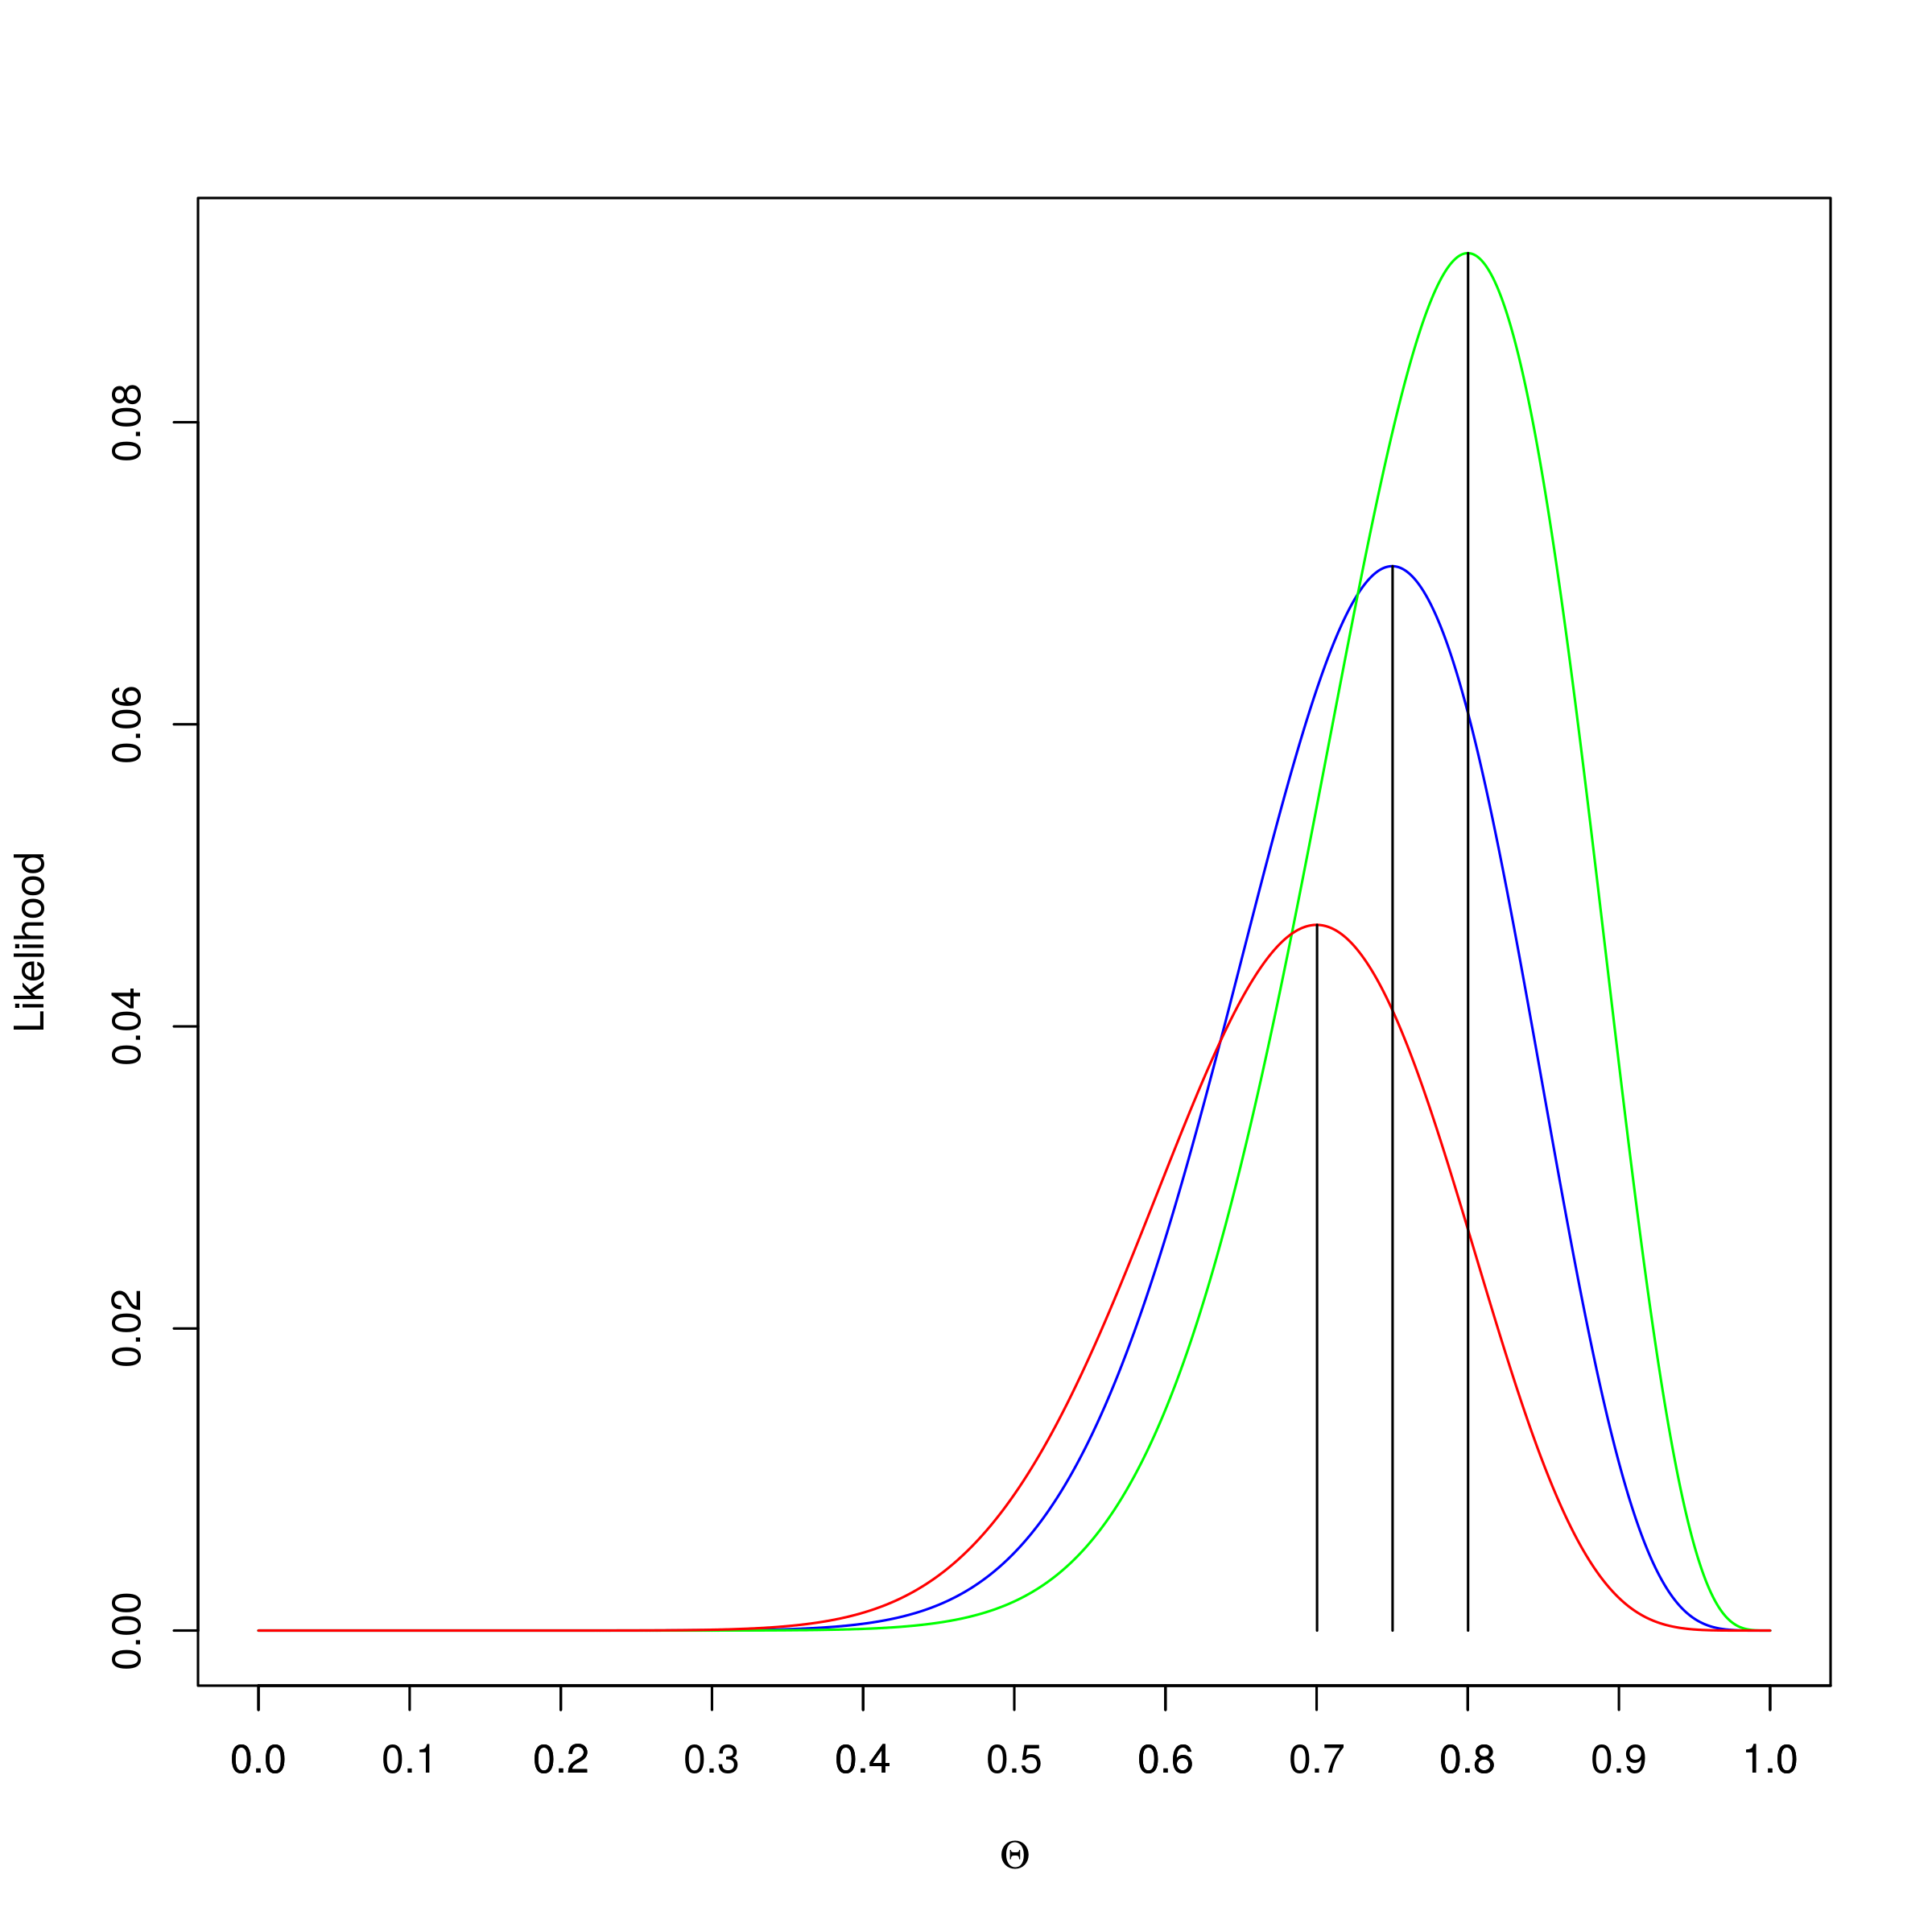
\includegraphics[scale=.3]{sparse_likelihood.png}
\caption{}
\label{fig:sparse_likelihood}
\end{subfigure}
~
\begin{subfigure}{.45\textwidth}
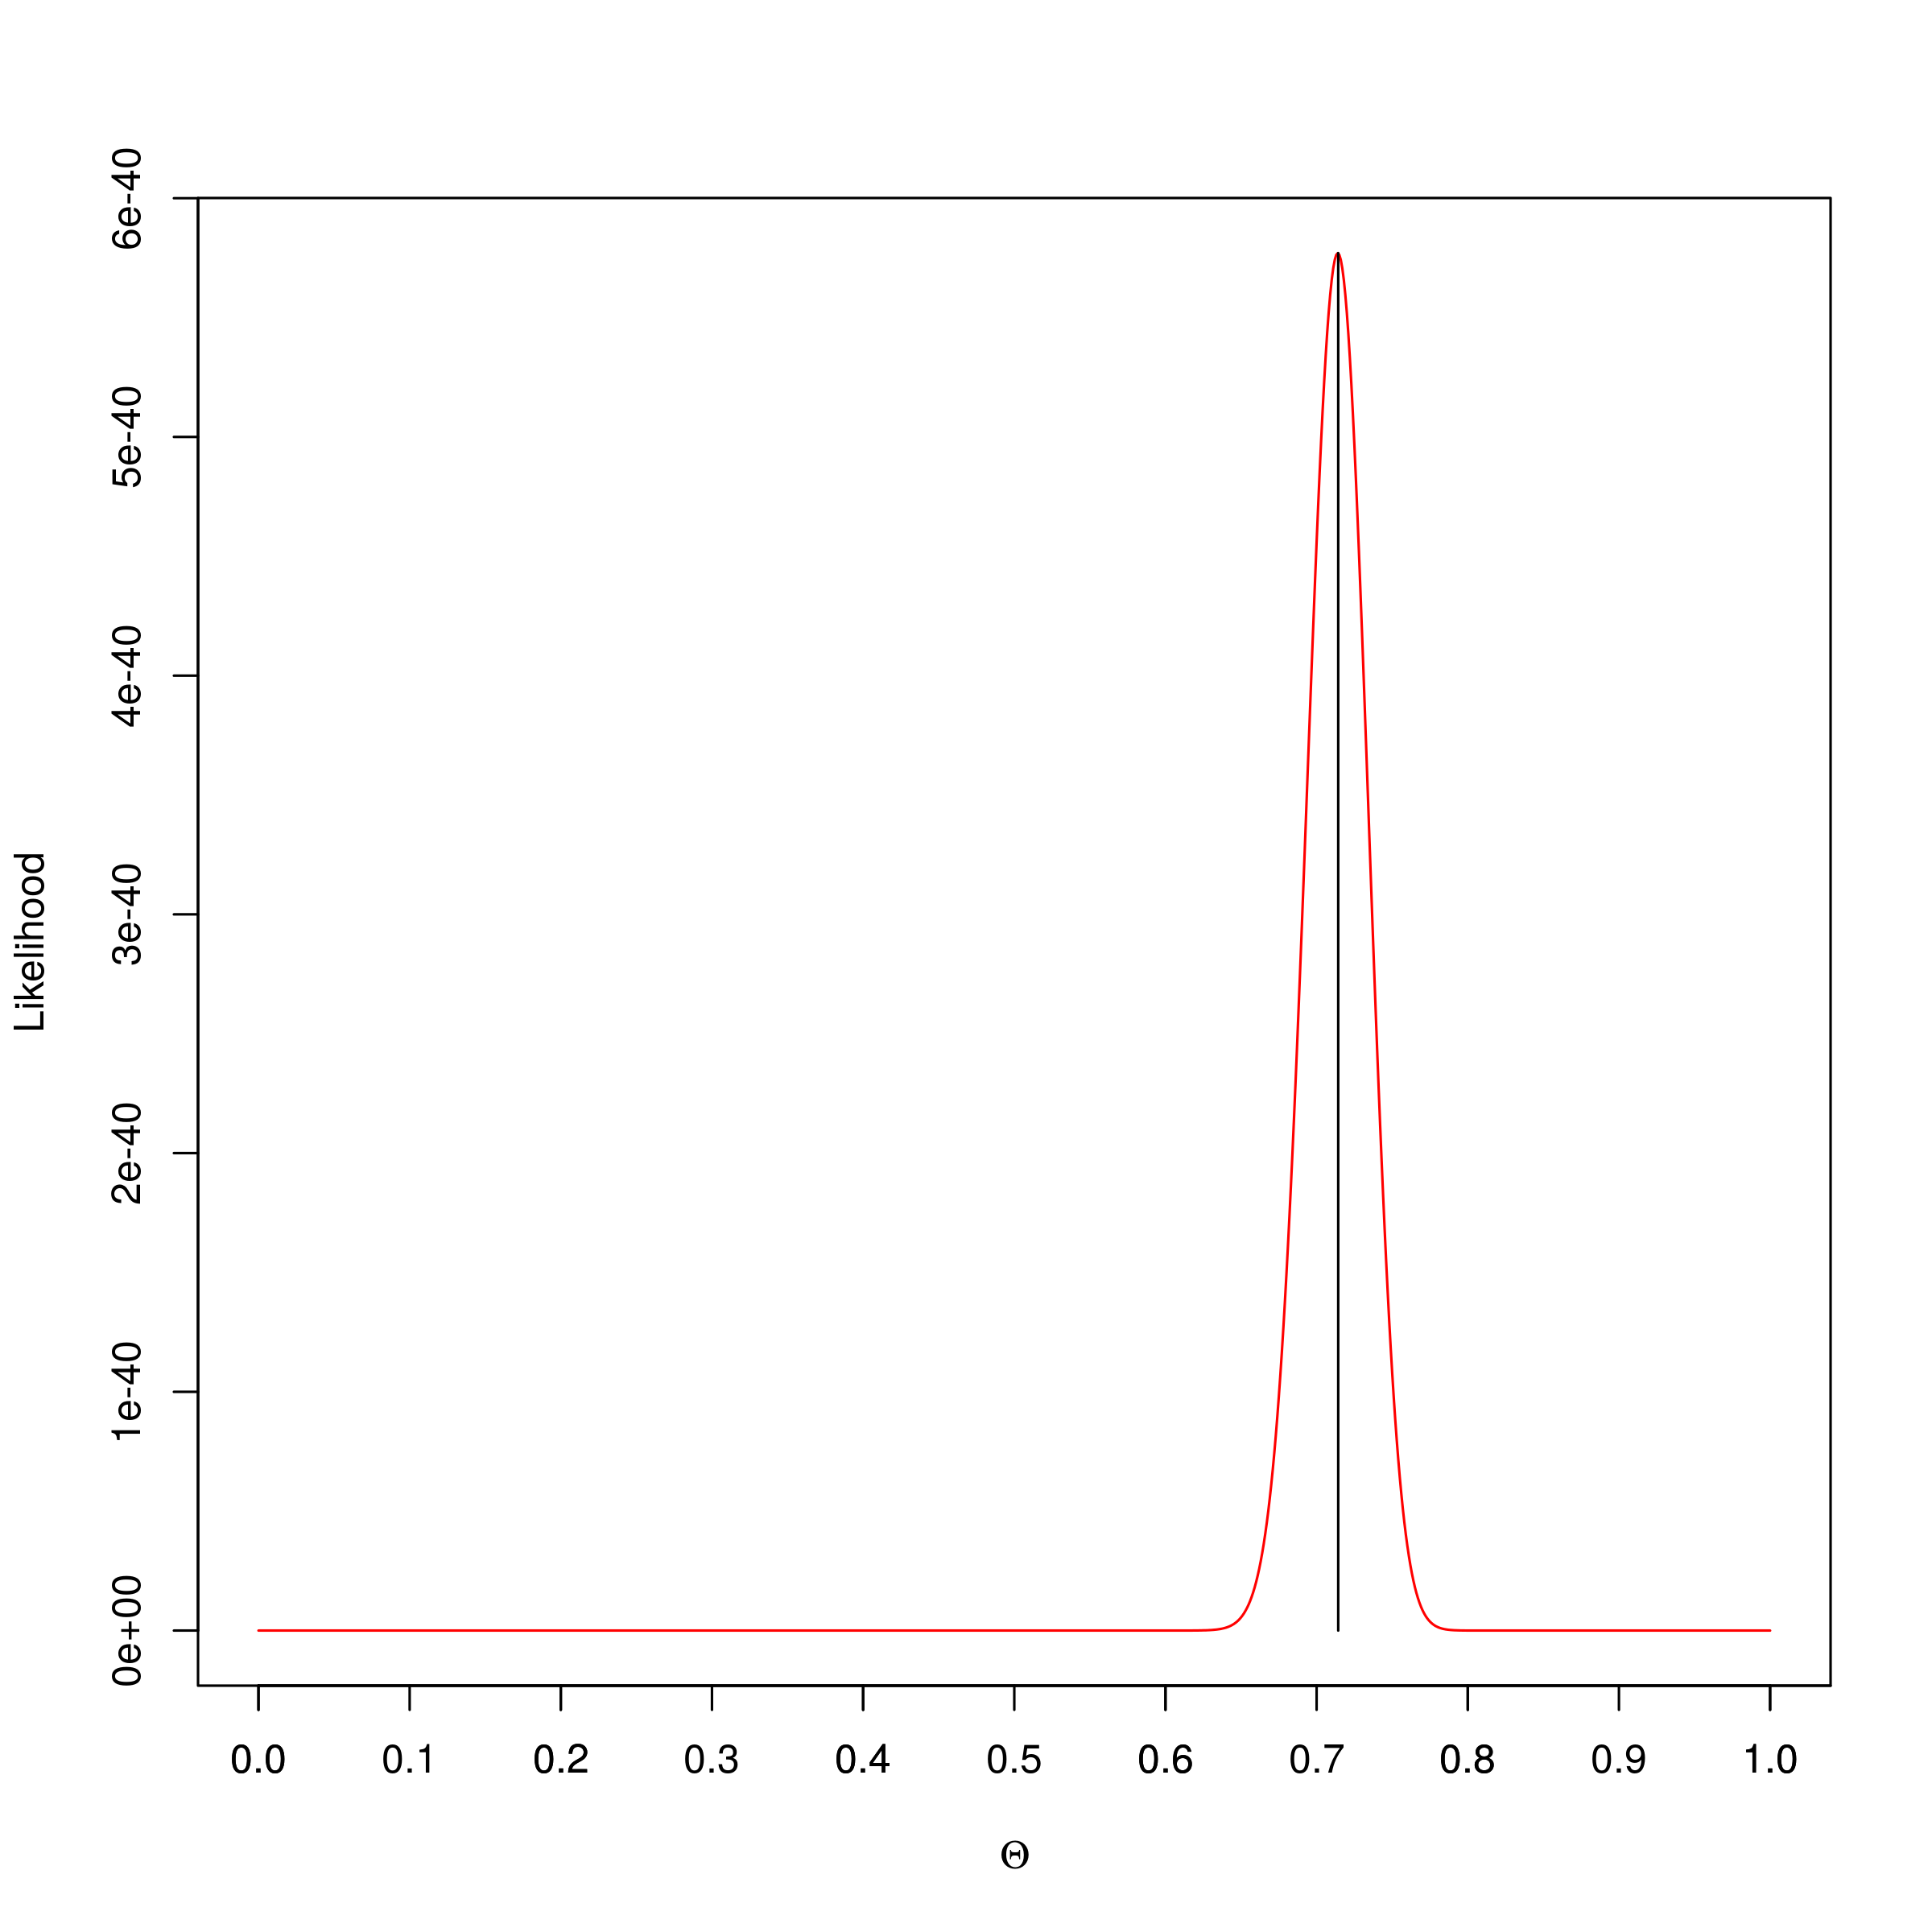
\includegraphics[scale=.3]{dense_likelihood.png}
\caption{}
\label{fig:dense_likelihood} 
\end{subfigure}
\caption{Plots of likelihood functions for different data samples. All data samples were randomly drawn
from a binomial distribution with parameters $ n=10 $ and $ \theta=0.7 $. Figure~\ref{fig:sparse_likelihood}
depicts the likelihood functions for data samples consisting of 2 draws each. The vertical lines indicate
at which value of $ \theta $ the likelihoods reach their maximums. Two draws contain relatively little
information about the underlying distribution and thus the likelihood function is fairly spread, indicating that there
are several parameter values that are about equally good.
Figure~\ref{fig:dense_likelihood}
shows the likelihood function for a data sample consisting of 50 draws. 50 draws convey much more information about the underlying distribution
and therefore the likelihood function is peaked around the MLE (which is also close to the true parameter $ 0.7 $. Deviating slightly from the MLE in his scenario
leads to a huge drop in likelihood, effectively ruling out a huge part of the parameter space as candidates for the true parameter.}
\label{fig:likelihood_plots}
\end{figure}

The maximum likelihood principle simply states that we should try to maximize the likelihood function of
our data, that is, we should pick the parameter value that achieves this maximisation. This parameter value
is known as the \textbf{maximum likelihood estimate} (or as maximum likelihood estimates if there are several). 

\begin{Definition}[Maximum Likelihood Estimate]
A maximum \\ likelihood estimate (MLE) for a parameter set~~$ \supp(\Theta) $ on a data sample $ x $ 
is a value $ \theta^{*} $ such that
$$ \theta^{*} = \underset{\theta}{\arg\max}\, \, L_{x}(\theta) $$
\end{Definition}

In Figure~\ref{fig:likelihood_plots} we have plotted some likelihood functions. They are based on data
samples that were randomly generated from a binomial distribution with parameters $ n=10 $ and 
$ \theta=0.7 $. The likelihood plots in Figure~\ref{fig:sparse_likelihood} are based on data sets of only
two samples, that is 20 i.i.d.\ Bernoulli trials. The plot in Figure~\ref{fig:dense_likelihood} is based on a 
data set of 50 samples, that is 500 i.i.d. Bernoulli trials. 
The vertical lines connect the maximum likelihood estimate
for each data set with its likelihood value. Notice the different scales of the two plots. The likelihood value depends on the
data size. Therefore, it does not make sense to compare likelihood values across data sets. After all, each data set comes with its own
likelihood function and the likelihood functions of different data sets are indeed different functions. This difference is also the
reason why the maximum likelihood principle tells us to only find the parameter value $ \theta $ at which the maximum of the
likelihood function is achieved. There is no point in even looking at the numerical likelihood value of that maximum.

Notice further that in Figure~\ref{fig:likelihood_plots}, there is only one MLE for each of these functions. We will shortly see why it is desirable for 
the likelihood function to only have one maximum.

Let us explain how to compute a MLE. By definition, the likelihood function maps the MLE to
one of its maximums. From calculus we know that the derivative of any differentiable function is 0 at the
function's maximums\footnote{Technically we also require that the function be defined on a closed 
(as opposed to open) interval. At this stage it is ok to assume that our parameter sets are always closed
intervals.}. Hence, all we need to do in order to find the MLE is to differentiate the likelihood 
function with respect to $ \theta $ and check where the derivative is 0. 
First, however, we need to write down the likelihood function.
Looking back at Definition~\ref{def:likelihood}, we recall that the likelihood is defined only
with respect to a probabilistic model. In order to write down a likelihood function, we need to first
define such a model. In other words, we have to define concrete likelihood functions on a case-by-case 
basis. We present one such case as an example below. Before we do so, let us note that for mathematical
convenience, one often uses the logarithm of the likelihood function instead of the likelihood function
itself. Taking the logarithm has two advantages: 1) logarithms turn products into sums and sums are often easier to handle
and 2) when using a computer, very small values may be rounded down to 0. Logarithms mitigate this problem
as they turn very small numbers into negative numbers that have rather large absolute values.

\begin{Definition}[Log-Likelihood]
For $n \in \mathbb{N} $ and a \emph{fixed} set of $n$ data points or observations $ x = x^{1}_{n} = x_1,x_2,\ldots,x_n $, we define the 
log-likelihood function over a 
family of distributions $ P_{x|\Theta} $ as 
$$ \mathcal{L}_{x}(\theta) := \log \left(L_{x}(\theta) \right) \ . $$
\end{Definition}

Notice that finding the maximum of the logarithm of any function $ f $ that only takes on positive values is the same as finding
the maximum of the original function $ f $. This is so because the logarithm function is strictly increasing, meaning that for any
two possible arguments $ x >y>0 $, we have $ \log(x) > \log(y) $ and hence, if $f(w) > f(z)$, we have $\log(f(w)) > \log(f(z))$.

In order to make it easier to find MLEs of your own, we give you a procedure that you can apply in most cases and
show you an example of how to use it.
\begin{enumerate}
\item Define a probabilistic model.
\item Write down the functional form of $ L_{x}(\theta) $ for the parameters of that model.
\item Write down $ \mathcal{L}_{x}(\theta) $.
\item Compute $ \frac{d}{d \theta} \mathcal{L}_{x}(\theta) $. This is also called the score function.
\item Solve $ 0 = \frac{d}{d \theta} \mathcal{L}_{x}(\theta) $ for $ \theta $.
\end{enumerate}

\paragraph{Example of finding the MLE} Assume we have to do market research for a clothing store in Amsterdam.
The store wants to expand its size and the manager wonders whether he should use the extra space to 
exhibit more men's or more women's clothing. To help him with this decision, we are going to count 
how many male and female customers are coming in on a given day. We treat the gender of each of the $n$ customers
as a random variable $ X_{i}$ and interpret $ X_{i} = 0 $ as male and $ X_{i} = 1 $ as
female. We assume that the underlying distribution that determines the gender of customers
is the same for all customers. We also assume that a customer's gender is independent of the gender of any
other customer. Hence, we stipulate that $ X_{i} \bot X_{j} $ whenever $ i \not = j $.

As an aside, notice that these assumptions are not without problems in real applications. 
The first assumption, that the gender
distribution is the same for all customers, may not always be justifiable. Depending on the time of the day,
it is possible that more men or women will come in. The second assumption, that the gender of one customer
does not depend on the gender of other customers, may also not always be true. If couples come to shop
at the store, then the gender of one partner will determine the gender of the other partner (in which
way the partners in a couple determine each other's genders depends on whether the couple is homo- or
heterosexual). For the sake of the example we will nevertheless assume that our assumptions hold true.

\textbf{Step 1:} As the day is over, we have observed $ k $ women and $ n-k $ men. Above, we postulated a model
according to which the
occurrences are distributed according a binomial distribution whose parameter $ n $ we already know: it
is simply the total number of our observations (a.k.a. the total number of customers who entered the shop 
that day). What we want in order to facilitate the manager's decision is to estimate $ \theta $, the
probability that a random customer is female. 

\textbf{Step 2:} Our likelihood function looks as follows:
\begin{equation}
L_{x}(\theta) = \binom{n}{k} \theta^{k} \times (1 - \theta)^{n-k} \ .
\end{equation}
As a mnemonic that $ \theta $ is unknown we can informally write
$$ L_{x}(\theta) = \binom{n}{k} ?^{k} \times (1-?)^{n-k} \ . $$

\textbf{Step 3:} We can now take the logarithm of our likelihood function.
\begin{align}
\log(L_{x}(\theta)) &= \log\left(\binom{n}{k} \theta^{k} \times \theta^{n-k} \right) \\
&= \log \left(\binom{n}{k}\right) + k\log(\theta) + (n-k)\log(1-\theta)
\end{align}

\textbf{Step 4:} To find the MLE, we first differentiate the log-likelihood with respect to $ \theta $.
\begin{align}
\frac{d}{d \theta} \mathcal{L}_{x}(\theta)
&= \frac{d}{d \theta} \log \left(\binom{n}{k}\right) + k \frac{d}{d \theta} \log(\theta) + (n-k) \frac{d}{d \theta} \log(1-\theta) \\
&= \dfrac{k}{\theta} - \dfrac{n-k}{1-\theta}
\end{align}

\textbf{Step 5:} Finally, we want to find a point where this derivative vanishes in order to find the maximum of $ \mathcal{L}_{x} $.
\begin{align}
0 &= \dfrac{k}{\theta} - \dfrac{n-k}{1-\theta} &\Leftrightarrow \\
\dfrac{n-k}{1- \theta} &= \dfrac{k}{\theta} &\Leftrightarrow \\
(n-k) \theta &= k (1 - \theta) &\Leftrightarrow \\
n\theta- k\theta &= k - k \theta &\Leftrightarrow \\
n\theta&= k &\Leftrightarrow \\
\theta &= \dfrac{k}{n}
\end{align}

And we are done! You know once and for all that the MLE for the parameter $\theta$ of \emph{any} binomial distribution with parameter $n$ (and having observed $k$ occurrences) is $ \frac{k}{n} $.

\begin{Exercise}
A coin is getting flipped 1000 times and comes up heads 600 times. According to the MLE, would you say that this coin is fair?
\end{Exercise}

Those who are already familiar with calculus may have felt a bit uncomfortable, because we simply state that setting the derivative of the log-likelihood
to 0 will give us a maximum of that function. In general, this technique will only give us an extremum which might as well be a minimum. How can we be so sure that
we really got a maximum? We will just do a proof by picture here and let you do the math. 

Take another look at Figure~\ref{fig:likelihood_plots}. Clearly, we only
see one maximum per function and that one is unique in all cases. 
What you cannot see in the plots is that the likelihood is never 0 for any $ \theta \in (0,1) $. It is just
really, really small, that is why it looks as if it was 0 in many places in the plot. What actually happens is that the likelihood is constantly decreasing as
$ \theta $ approaches 0 and 1. This constant decrease implies that the derivative is not equal to $ 0 $ anywhere other than at the maximum.

Finally, notice that the likelihood is only equal to 0 when $ \theta = 0 $ or $ \theta = 1 $. 
Thus, the likelihood function does indeed have two minima. However, these 
occur at the boundary points of the interval $ [0,1] $ and since we just stated that $ L_{x}(\theta) $ is constantly decreasing as $ \theta $ approaches those points,
we can safely conclude that the maximum does not lie on the boundary points. Hence, the only point at which the
derivative of the likelihood function of the binomial distribution is $ 0 $ is at the sole maximum.

We have mentioned above that having only one maximum is a desirable property. If we want to find the MLE, we have but one choice in this case. If there were
several maxima, we would have to compute all of them and pick amongst them. If there are two maxima that have equal likelihood values, we have no way of choosing
between them and thus no way of determining the single best parameter estimate. Moreover, we will encounter situations in the next chapter where it is very hard (if not
impossible) to find the global MLE (i.e.\ the MLE at the highest maximum).

You may rightfully wonder what distributions have the desirable property of only having one maximum in their likelihood functions. It turns out that those are
exactly the distributions in the \href{https://en.wikipedia.org/wiki/Exponential_family}{exponential family}. The link includes a list of those distributions and
you will be happy to see that most commonly used distributions are members of the exponential family and thus their likelihoods only have one maximum. Another feature of exponential family distributions is that
they all have sufficient statistics. Hence, whenever we are doing maximum likelihood estimation for 
an exponential family distribution, all we need to know about the data are the sufficient statistics. This
point will become important in the following chapter.

\begin{Exercise}
You are given some likelihood function $ L_{x} $ for the binomial distribution along with its MLE $ \theta^{*} $. Show rigorously that $ \theta^{*} $ is indeed
a maximum. That is, show that $ \mathcal{L}_{x}''(\theta^{*}) < 0 $, where $ \mathcal{L}_{x}'' $ is the second derivative of the log-likelihood function.
\end{Exercise}

 
\section{Maximum a Posteriori Estimation}

Recall that in Section~\ref{parameterEstimation} we set ourselves the goal of finding a good parameter estimate from the posterior distribution over parameters.
Let us say that the best parameter estimate is the one with the highest posterior probability. Then the question is: do we actually accomplish our goal with the MLE?
Does the MLE give us the parameter with the highest posterior probability? Unfortunately, the general answer is no, which becomes evident from Bayes' rule.
\begin{equation}
\underset{\theta}{\arg\max}~P(\Theta = \theta| X=x) = \underset{\theta}{\arg\max}~P(X=x|\Theta=\theta) \times P(\Theta = \theta)
\end{equation}

The MLE only maximises over the likelihood term but not over the prior! Hence it will in general be different from the \textbf{maximum a posteriori} estimate.

\begin{Definition}[Maximum a posteriori estimate]
A maximum a posteriori (MAP) estimate for a parameter set~~$\supp(\Theta)$ on a data sample $ x $ 
is a value $ \theta^{*} $ such that
$$ \theta^{*} = \underset{\theta}{\arg\max}\, \, P(\Theta = \theta| X=x) \ . $$
\end{Definition}

The MAP estimate can be derived with exactly the same steps as the MLE. However, parameters are usually real values which means that distributions over them
are continuous distributions. Since we have not dealt with continuous distributions in this course, we will stop just short of actually imposing
(non-uniform) prior distributions over parameters and computing MAP estimates.

Notice that up to now, we justified the maximum likelihood principle merely from intuition by postulating that high likelihood should somehow be an indicator for
good parameter values. We will now justify the maximum likelihood principle more formally, by showing that the MLE is just a special kind of MAP estimate. Since
this realisation implies that under certain condition the MLE will also have the highest posterior probability, we can safely argue for the MLE based on its posterior probability.

Let us assume that our prior distribution $ P_{\Theta} $ over parameters is uniform. Then we can write the MAP estimator\footnote{If you know some continuous probability
theory: the MAP estimate is taken on the posterior density function in this case since the distribution over parameters is continuous.} as
\begin{align}
&\underset{\theta}{\arg\max}\, \, \frac{\partial}{\partial\theta} \log (P(\Theta = \theta| X=x)) \\
= &\underset{\theta}{\arg\max}\, \, \frac{\partial}{\partial\theta}\log (P(X=x|\Theta=\theta) \times P(\Theta = \theta)) \\
= &\underset{\theta}{\arg\max}\, \, \frac{\partial}{\partial\theta}\log (P(X=x|\Theta=\theta)) + \log(P(\Theta = \theta)) \label{eq:posteriorDiff} \\
= &\underset{\theta}{\arg\max}\, \, \frac{\partial}{\partial\theta}\log (P(X=x|\Theta=\theta)) \label{eq:MLE=MAP} \, ,
\end{align}
where we used the uniformity of $\Theta$ to get from \eqref{eq:posteriorDiff} to \eqref{eq:MLE=MAP}. We can neglect $ \log(P(\Theta = \theta) $ when finding the maximum, because if we add a constant to all likelihood values, the MLE will not change.

This derivation tells us that if we choose a uniform parameter prior, the MLE will be the MAP estimate. Hence, what we are actually assuming whenever we choose the MLE as
our parameter estimate, is that our prior over parameters is uniform. This is a very strong assumption to make and one may rightfully criticise the maximum likelihood principle because of this assumption (actually one should).

Let us conclude this section by saying that for the rest of this course we will make the assumption that we are using uniform parameter priors with justification.
This means that we can safely use the MLE in order to find the parameter value with the highest posterior probability.


\section*{Further reading}
If your calculus is a bit rusty or you have never taken a calculus class before, you should consult 
\href{https://www.coursera.org/learn/calculus1}{OSU's excellent (and very fun) online course} which allows you to learn at your own pace. The course also comes with
\href{https://mooculus.osu.edu/handouts}{a lecture script} that contains many insightful examples and exercises. Let us emphasise that doing statistics (including
machine learning) without a solid understanding of calculus is close to impossible.

If you are looking for a good introduction to
parameter estimation that covers everything we have discussed here and also goes a considerable stretch further, we refer you to 
\href{http://www.arbylon.net/publications/text-est.pdf}{Gregor Heinrich's widely cited tutorial}. Heinrich's examples come from text modelling but the techniques he
describes can be applied anywhere. One of the model he discusses, \href{https://en.wikipedia.org/wiki/Latent_Dirichlet_allocation}{Latent Dirichlet Allocation}, originates
from text modelling but has wide-spread applications in biology, as well.


%%% Local Variables:
%%% mode: latex
%%% TeX-master: "chapter5"
%%% End:
